\section{Felder}
Zusammenhang Elektrostatik $\Leftrightarrow$ Magnetostatik\\
\[ \vec{J} = \kappa \vec{E} \]

\subsection{E-Felder an Grenzflächen}
\textbf{Dielektrische Grenzfläche}\\
\begin{tabularx}{0.45\textwidth}{>{\hsize=.3\hsize}X>{\hsize=.5\hsize}X}
    Querschichtung:   & $D_{1n} = D_{2n}$                                                                                                      \\
                      & ${\displaystyle\oiint} \vec{D} \cdot d \vec{a} = 0$                                                                    \\
    Längsschichtung:  & $E_{1t} = E_{2t}$                                                                                                      \\
                      & $ {\displaystyle\oint} \vec{E} \cdot d \vec{s} = 0$                                                                    \\
    Schrägschichtung: & $ \frac{tan( \alpha_1)}{tan( \alpha_2)} = \frac{E_{1t}/E_{1n}}{E_{2t}/E_{2n}} = \frac{ \varepsilon_1}{\varepsilon_2} $
\end{tabularx}

\textbf{Grenzfläche dielektrischer Leiter}\\
\begin{tabularx}{0.45\textwidth}{>{\hsize=.3\hsize}X>{\hsize=.5\hsize}X}
    Längsschichtung: & $E_{1t} = E_{2t}$                                   \\
                     & ${\displaystyle\oint} \vec{E} \cdot d \vec{s} = 0$  \\
    Querschichtung:  & $D_{1n} = \frac{Q}{A}$                              \\
                     & ${\displaystyle\oiint} \vec{D} \cdot d \vec{a} = Q$
\end{tabularx}

\textbf{Grenzfläche an magn. Feldern}\\
\begin{tabularx}{0.45\textwidth}{>{\hsize=.3\hsize}X>{\hsize=.5\hsize}X}
    Querschichtung:   & $B_{1n} = B_{2n}$                                                  \\
                      & ${\displaystyle\oiint} \vec{B} \cdot d \vec{a} = 0$                \\
    Längsschichtung:  & $H_{1t} = H_{2t}$                                                  \\
                      & ${\displaystyle\oint} \vec{H} \cdot d \vec{s} = 0$                 \\
    Schrägschichtung: & $\frac{tan( \alpha_1)}{tan( \alpha_2)} = \frac{ \mu_1 }{ \mu_2 } $
\end{tabularx}

\subsection{Elektrostatik}
ist ein wirbelfreies Feld. Elek. Ladungen sind Quellen des Feldes.
\begin{align*}
    \opdiv \vec{D} = \nabla \cdot \vec{D}  & = \rho       \qquad          \vec{D} = \varepsilon \vec{E} \\
    \oprot \vec{E} = \nabla \times \vec{E} & = 0          \qquad          = \oprot \opgrad E            \\
    \vec{E}                                & =- \opgrad \varphi
\end{align*}
\subsubsection{Potetialgleichung}
\[
    \opdiv \opgrad \varphi = - \dfrac{\rho}{\varepsilon}
\]
\paragraph{$\qquad \Rightarrow$ Poisson-Gleichung}
mit $\rho = 0 \Rightarrow$ \textbf{Laplace-Gleichung}
\begin{align*}
    \Delta \varphi + \underbrace{ \dfrac{\opgrad \varepsilon \cdot \opgrad \varphi}{\varepsilon}}_{= 0\texttt{, wenn homogen}}
     & = - \dfrac{\rho (x, y, z)}{\varepsilon} \\
    \frac{d^2 \varphi}{d x^2} + \frac{d^2 \varphi}{d y^2} + \frac{d^2 \varphi}{d z^2}
     & = - \dfrac{\rho (x, y, z)}{\varepsilon}
\end{align*}

\subsubsection{Green'sche Funktionen}
\paragraph*{Potential einer Punktladung}
\[ \varphi (r) = \dfrac{Q}{4 \pi \varepsilon \cdot r} \]

\paragraph*{E-Feld einer Punktladung}
\[ \vec{E}(r) = \dfrac{Q}{4 \pi \varepsilon \cdot r^2} \]

\paragraph*{D-Feld einer Punktladung}
\[ \vec{D}(r) = \dfrac{Q}{4 \pi \cdot r^2} \]

\paragraph*{Potentialfeld einer Ladungsverteilung}
mit $\varphi(\infty)=0$
\[
    \varphi(x, y, z)=\frac{1}{4 \pi \varepsilon} \iiint_{V^{\prime}}
    \frac{\rho\left(x^{\prime}, y^{\prime},
        z^{\prime}\right)}{\left|\vec{r}-\vec{r}^{\,\prime}\right|} \mathrm{d}
    V^{\prime}
\]

mit der Green'schen Funktion $G\left(\vec{r}, \vec{r}^{\,\prime}\right)=\frac{1}{4 \pi \varepsilon\left|\vec{r}-\vec{r}^{\,\prime}\right|}$
\[\varphi(x, y, z)=\iiint_{V^{\prime}} G\left(\vec{r}^{\,\prime} \vec{r}^{\,\prime}\right) \rho\left(\vec{r}^{\,\prime}\right) \mathrm{d} V^{\prime}\]


\subsection{Magnetostatik}
ist ein Wirbelfeld, quellenfrei und hat geschlossene Feldlinien.
\begin{align*}
    \oprot \vec{H} = \nabla \times \vec{H} & = \vec{J}  \qquad \vec{B} = \mu \vec{H}   \\
    \opdiv \vec{B} = \nabla \cdot \vec{B}  & = 0        \qquad = \opdiv \oprot \vec{B}
\end{align*}

\paragraph*{Coulomb-Eichung}
\begin{align*}
    \Delta \vec{A} & = - \mu \vec{J}  \\
    \vec{B}        & = \oprot \vec{A}
\end{align*}

\subsubsection{Vektorpotential in Abhängigkeit von der Stromdichte}
\[ \vec{A}(x, y, z)=\frac{\mu}{4 \pi} \iiint_{V^{\prime}} \frac{\vec{J}\left(x^{\prime}, y^{\prime}, z^{\prime}\right)}{\left|\vec{r}-\vec{r}^{\,\prime}\right|} d V^{\prime} \]

\subsubsection{Biot-Savart-Gesetz}
\[
    \vec{H}=\frac{I}{4 \pi} \oint_{C^{\prime}} \opgrad \frac{1}{\left|\vec{r}-\vec{r}^{\,\prime}\right|} \times \mathrm{d} \vec{s}^{\,\prime}
\]

mit $\opgrad \frac{1}{\left|\vec{r}-\vec{r}^{\,\prime}\right|}=-\frac{\vec{r}-\vec{r}^{\,\prime}}{\left|\vec{r}-\vec{r}^{\,\prime}\right|^{3}}$

\[
    \vec{H}=\frac{I}{4 \pi} \oint_{C^{\prime}} \frac{\mathrm{d} \vec{s}^{\,\prime} \times\left(\vec{r}-\vec{r}^{\,\prime}\right)}{\left|\vec{r}-\vec{r}^{\,\prime}\right|^{3}}
\]

$\vec{r}:$ Aufpunkt $\quad \vec{r}^{\,\prime}:$ Quellpunkt


\subsection{Skineffekt}

\makebox[0pt][l]{
    \begin{minipage}{\columnwidth}
        \centering
        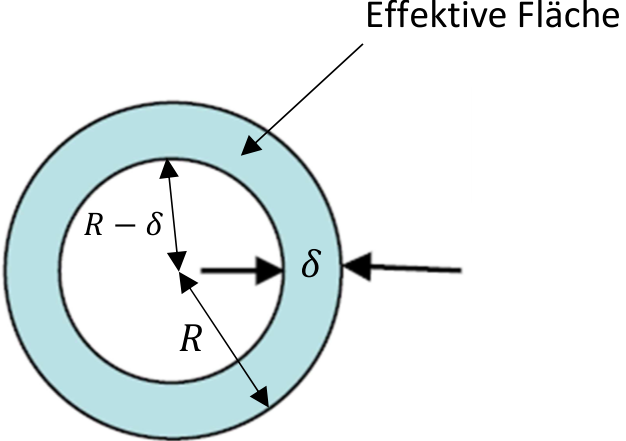
\includegraphics[width=.4\columnwidth]{Figures/Skineffekt.png}\\
        \hspace{-5em}
        {\footnotesize$\sigma/\kappa$ : Leitfähigkeit. $[\si{A/Vm}] = [\si{1/\Omega m}]$}
    \end{minipage}
}

\begin{description}
    \item Äquivalente Leiterschichtdicke (Amp: $A \cdot \frac{1}{e}$):
        \[
            \delta = \frac{1}{\sqrt{\pi\mu\sigma f}} = \sqrt{\frac{2}{\omega\mu\sigma}} \qquad \left[ m \right] \\
        \]

    \item Widerstand/ Oberflächenwiderstand:
          \begin{align*}
              R_{r\ll\delta}     & = \frac{l}{\sigma \cdot A_{\texttt{eff}}} \\
              R_{r\approx\delta} & =\dfrac{4l}{\sigma \pi d^{2}}             \\
              R_F                & = \dfrac{1}{\sigma \delta}
          \end{align*}

    \item \textbf{Feldstärke} verglichen mit der Oberfläche:
          \begin{align*}
              H\left( x,t\right) & =H_{0}\cdot e^{^{-x}/_\delta}\cdot \cos \left( \omega t-\dfrac{x}{\delta}\right)
          \end{align*}
          analog für $E$-Feld

    \item \textbf{Leistung} verglichen mit der Oberfläche:
          \begin{align*}
              P\left( x,t\right) & =\dfrac{1}{2} \cdot E_{0}\cdot e^{^{-x}/_\delta}\cdot H_{0}\cdot e^{^{-x}/_\delta}
          \end{align*}

    \item Amplitude und Phase bezogen auf $\delta$:
          \begin{align*}
              \text{Amplitude: } x   & =\delta \cdot \ln(\text{Dämpfung[ ]}) \\
              \text{Phase: } \varphi & = -\frac{x}{\delta}
          \end{align*}

    \item Effiktive Fläche:
          \begin{align*}
              A_{\texttt{eff}} & = A_{\texttt{ges}} - A_{\sigma} = R^2\pi-(R-\sigma)^2\pi \\
                               & =2\cdot \pi \delta \left( R-\dfrac{\delta }{2}\right)
          \end{align*}
\end{description}

Wenn die Länge nicht gegeben ist oder nach Wieviel \% nimmt der Widerstand bei
einer bestimmten Frequenz, kann dies mit der folgenden Formel berechnet werden:

\begin{description}
    \item Bessel-Funktion:
          \begin{align*}
              \frac{R_{AC}}{R_{DC}} & =
              \begin{dcases}
                  1 + \frac{1}{3}x^4              & \text{für} \qquad x > 1 \\
                  x + \frac{1}{4} + \frac{3}{64x} & \text{für} \qquad x < 1 \\
              \end{dcases} \\
              \frac{R_{AC}}{R_{DC}} & =
              \begin{dcases}
                  x^2\left( 1-\frac{x^4}{6} \right)                               & \text{für} \qquad x > 1 \\
                  x- \frac{1}{4} + \frac{3}{64x} + \frac{1}{4} + \frac{3}{128x^2} & \text{für} \qquad x < 1 \\
              \end{dcases}
          \end{align*}
          \[
              \boxed{x=\frac{r_0}{2\delta}} \qquad r_0 \hat{=} \textnormal{ Außendurchmesser}
          \]
\end{description}
\newpage
